\documentclass{article}
\usepackage[left=3cm,right=3cm,
    top=2cm,bottom=2cm,bindingoffset=0cm]{geometry}
\usepackage{graphicx} % Required for inserting images

\usepackage[english, russian]{babel}
\usepackage[T2A]{fontenc}			% кодировка
\usepackage[utf8]{inputenc}			% кодировка исходного текста
\usepackage{amsmath,amsfonts,amssymb,amsthm,mathtools}

\setlength{\parindent}{0pt}			% убрать отступ

\title{\textbf{Лабораторная работа 1.4.5.} \linebreak
ИЗУЧЕНИЕ КОЛЕБАНИЙ СТРУНЫ}
\author{Попова Софья Б04-401}
\date{November 2024}

\begin{document}

\maketitle

\section*{Цель работы}
Исследование зависимости частоты колебаний струны от величины нятяжения, а также условий установления стоячей волны, получающейся в результате сложения волн, идущих в противоположных направлениях.

\section*{Оборудование}
Рейка со струной, звуковой генератор, постоянный магнит, разновесы.

\section*{Теоретическая часть}
Гибкость струны является следстваием ее большой длины в ставрениии с малыми поперечными размерами. Даже струны, изготовленные из жестких материалов, практически не сопротивляются изгибу, что позволяет пренебречь изгибными напряжениями. За счет натяжения струна вытягивается практически в прямую линию, сила нятяжения значительно первосходит вес струны, что позволяет пренебречь силами тяжести.

По волновому уравнению скорость распространения поперечной волны на струне равна (где $F$ - сила натяжения струны, $\rho_l$ - масса струны на единицу длины):
\begin{equation}
    u =\sqrt{\frac{F}{\rho_l}}
\end{equation}

При заданной частоте $\nu$ длина волны равна $\lambda$:
\begin{equation}
    \lambda = \frac{u}{\nu}
\end{equation}

Частоты собственных колебаний струны определяются формулой (где $l$ - длина волны, $n$ - число полуволн):
\begin{equation}
    \nu_n=n\frac{u}{2l}
\end{equation}
Эту формулу будем использовать для теоретического рассчета частоты гармоник.

\newpage

\section*{Экспериментальная часть}
Проведем предварительные рассчеты:

\

Сила натяжения нити $T = Mg$, где M = суммарная масса подвеса и изначальных грузиков. 

\ \ \ \ \ \ \ \ $M = 1012,7$г

\ \ \ \ \ \ \ \ $\rho = 568,4$ мг/м $= 0,5684$ г/м

Тогда: 

\ \ \ \ \ \ \ \ $u = \sqrt{\frac{M\cdot g}{\rho}}\approx 132,14$ м/с

Длина струны L (рекомендованное значение - 50 см) $= 50 \pm 0,05$ см. Рассчитаем частоту основной гармоники по формуле (3):

\ \ \ \ \ \ \ \ $\nu_1 = 1\cdot\frac{u}{2L} \approx 132$ Гц

\

Включим в сеть звуковой генератор, установим на нём синусоидальный тип сигнала. Установим регистрирующий датчик в центре под струной (в месте пучности). Убедиждаемся, что сигнал с выхода генератора подаётся на возбуждающий датчик. Устанавливаем на генераторе рассчитанную частоту $\nu_1$

\

Медленно изменяя частоту генератора в пределах $\nu_1 \pm 5$ Гц, добиваемся возбуждения стоячей волны с максимальной амплитудой регистрируемого сигнала на осциллографе, записываем значение частоты в табл.1

\

Увеличим частоту генератора в 2 раза и аналогичным образом определим частоту $\nu_2$, при которой амлпитуда колебаний достигает максимума. Проведём такое же измерение для 3-9 нечетных гармоник. Результат - в табл.1

\

Проведем измерения для еще 4 четных гармоник. Теперь посередине струны находится узел волны, поэтому регистрирующий датчик стоит сместить в сторону пучности. Результаты - в табл.1

\begin{table}[h]
    \centering
    \begin{tabular}{|c|c|c|c|c|c|c|c|c|c|}
    \hline
         Гармоника & $\nu_1$ &  $\nu_2$ &  $\nu_3$ &  $\nu_4$ &  $\nu_5$ &  $\nu_6$ &  $\nu_7$ &  $\nu_8$ &  $\nu_9$ \\
    \hline
         Частота & 136,49 & 273,28 & 409,7 & 549,2 & 685,1 & 826,2 & 967 & 1105 & 1250 \\
    \hline
    \end{tabular}
    \caption{масса грузиков = 1012,7 г}
\end{table}

Повторим измерения для других значений $T$. Натяжение нити будем изменять подвешивая дополнительные грузы к нити. Результаты измерений указаны в таблице 2.

\begin{table}[h]
    \centering
    \begin{tabular}{|c|c|c|c|c|c|c|c|c|c|c|}
    \hline
         Масса груза & Гармоника & $\nu_1$ &  $\nu_2$ &  $\nu_3$ &  $\nu_4$ &  $\nu_5$ &  $\nu_6$ &  $\nu_7$ &  $\nu_8$ &  $\nu_9$ \\
         1351,7 г & Частота & 158,2 & 315,4 & 474,3 & 632,5 & 789,2 & 948,2 & 1110 & 1266 & 1427 \\
    \hline
         Масса груза & Гармоника & $\nu_1$ &  $\nu_2$ &  $\nu_3$ &  $\nu_4$ &  $\nu_5$ &  $\nu_6$ &  $\nu_7$ &  $\nu_8$ &  $\nu_9$ \\
         1844,9 г & Частота & 181 & 364 & 548,3 & 731,9 & 915,5 & 1098 & 1284 & 1469 & 1651 \\
    \hline
         Масса груза & Гармоника & $\nu_1$ &  $\nu_2$ &  $\nu_3$ &  $\nu_4$ &  $\nu_5$ &  $\nu_6$ &  $\nu_7$ &  $\nu_8$ &  $\nu_9$ \\
         2327,3 г & Частота & 202 & 408,2 & 611,6 & 815,5 & 1020 & 1222 & 1430 & 1637 & 1843 \\
    \hline
         Масса груза & Гармоника & $\nu_1$ &  $\nu_2$ &  $\nu_3$ &  $\nu_4$ &  $\nu_5$ &  $\nu_6$ &  $\nu_7$ &  $\nu_8$ &  $\nu_9$ \\
         2821,7 г & Частота & 224 & 450,5 & 672,6 & 899,9 & 1126 & 1351 & 1577 & 1805 & 2032 \\
    \hline
    \end{tabular}
    \caption{Данные измерений при разных Т}
\end{table}

По полученным данным построим график зависимости частоты резронанса от n (рис.1)

\begin{figure}[h]
    \centering
    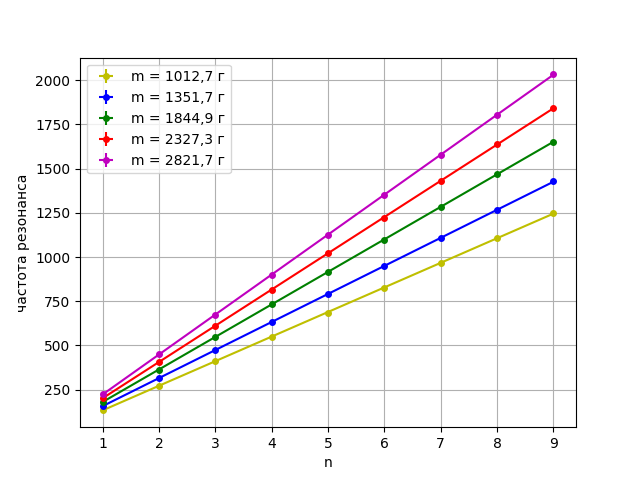
\includegraphics[width=1\linewidth]{5 lines.png}
    \caption{Графики зависимости $\nu_n(n)$}
\end{figure}

\newpage
Определим по наклону графика $u$ скорость волн в струне при каждом $T$ по формуле (3): $$\nu_n = n\frac{u}{2l} \ \ \ \ \ u=\frac{\nu_n \cdot2l}{n}$$

$u_1 = 137,4$ м/с.  \ Теоретическое значение: 132,21 м/с \ Разница составляет: $\frac{137,4-132,21}{137,4} \approx 0,038 (3,8\%)$

$u_2 = 158,1$ м/с.  \ Теоретическое значение: 152,74 м/с \ Разница составляет: $\frac{158,1-152,74}{158,1} \approx 0,034 (3,4\%)$

$u_3 = 182,8$ м/с.  \ Теоретическое значение: 178,44 м/с \ Разница составляет: $\frac{182,8-178,44}{182,8} \approx 0,024 (2,4\%)$

$u_4 = 203,9$ м/с.  \ Теоретическое значение: 200,42 м/с \ Разница составляет: $\frac{203,9-200,42}{203,9} \approx 0,017 (1,7\%)$

$u_5 = 225$ м/с. \ \ \ \ Теоретическое значение: 220,68 м/с \  Разница составляет: $\frac{225-220,68}{225} \approx0,019 (1,9\%)$

\

По полученным данным построен график зависимости квадрата скорости волны от силы натяжения нити (рис.2). По наклону прямой, по формуле (1) определим $\rho_l$: $$u^2 = \frac{F}{\rho_l} \ \ \ \rho_l = \frac{F}{u^2}$$

$\rho_l = 0,5383$ г/м = $538,3$ мг/м \ \ \ погрешность = \sqrt{(\frac{0,05}{1012,7})^2+2(\frac{0,038\cdot136,5}{136,5})^2} \approx 0,054 \ (5,4\%)

Значение, указанное на установке: $568,4$ мг/м \ \ Разница $\approx 5,3\%$

\begin{figure}[h]
    \centering
    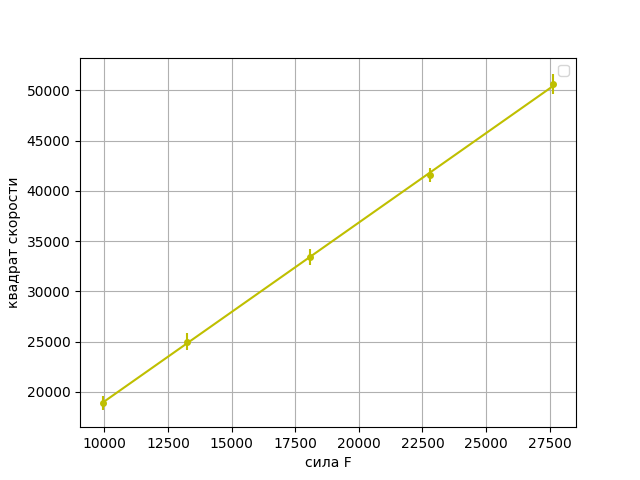
\includegraphics[width=1\linewidth]{2.png}
    \caption{График зависимости $u^2(F)$}
\end{figure}



\newpage
\section*{Вывод}

Во время выполнения работы было подтверждено несколько теоретических зависимостей между физическими величинами. Подтверждена формула для определения частот гармоники струны и формула для определения скорости распространения волны в твердом теле под действием внешней силы.

Полученные графики имеют вид, предсказанный теоретически. 

С точностью $ \varepsilon_{\rho_{l}} = 5,4\%$ определена линейная плотность струны, значение которой, в апределах погрешности, совпало со значением, указанным на установке.
	
\end{document}
